 

\chapter[Hijacked constructions in L2 Acquisition]{Hijacked constructions in Second Language Acquisition: Implications for Sri Lanka Malay}
\chapterauthor{Ian Smith}{York University, Toronto}

% \begin{abstract}
% Grammar development in creolization and contact-induced change without creolization may lead to similar-looking results. Inasmuch as creolization is language is similar to untutored Second Language Acquisition and involves L1 $>$ L2 influence \citep{Siegel2008}, it is more likely to display the results of \textit{hijacked} grammatical elements -- elements whose grammatical and semantic status in the lexifier is very different from their status in the creole. Hijacked constructions are much rarer in other types of language development, and in particular, in contact situations involving L1 $<$ L2 influence rather than L1 $>$ L2 influence. Therefore, creoles are hypothesized to be historically distinct from non-creoles in that they more frequently exhibit hijacked constructions.
% 
% This paper applies the above hypothesis to de-verbal nominalizations in four languages in contact with Tamil: two non-creoles (Sinhala, Sourashtra) a creole (Sri Lanka Portuguese) and a language of disputed status (Sri Lanka Malay). The former two exhibit calqued constructions, the creole exhibits a hijacked construction typical of untutored SLA, and Sri Lanka Malay has repurposed a pragmatically compatible but syntactically incongruent morpheme \textit{yang}. Finally, the details of the spread of de-verbal nominalizations demonstrate that syntactic borrowing need not replicate the source construction in every detail.
% 
% \end{abstract}


\section{Introduction}

Most creolists accept that there is a cline between creole and non-creole. Categories of contact-languages are, like most human categories, fuzzy-edged and centred on abstract \textit{prototypes}.\footnote{I
 would like to acknowledge the support of the Social Sciences and Humanities Research Council for fieldwork on Sri Lanka Portuguese (1974-5) and Sourashtra (1989-90; 1992). I am grateful to Mohamed Jaffar, B.A. Hussainmiya, and Romola Rassool for their assistance with Sri Lanka Malay, to the late Ronald Rosario and Richard Starack for their assistance with Sri Lanka Portuguese, to Richard Starack, Jothy Jeeveratnam for assistance with Sri Lanka Tamil, to Mohamed Jaffar for assistance with Shonam, to Ranjhani Raghunathan for assistance with Indian Tamil, to K. S. Shanti, A. R. Kumar, K. Pasumpon, O. K. Ramanandam, V. V. Ramlakshmanji, R. R. Parimalam, and N. M. Omprakash for assistance with Sourashtra, and to Romola Rassool for assistance with Sinhala. Thanks to Bill Foley for comments on an oral presentation of a related paper. 
 Standard abbreviations are used as prescribed by the Leipzig glossing rules and the list of abbreviations provided in this book.
Additional abbreviations are as follows: 
%  \textsc{adjz} adjectivalizer; 
%  \textsc{advz} adverbializer; 
%  \textsc{aug} augment; 
%  \textsc{exper} experiential; 
%  \textsc{cnj} conjunction; 
%  \textsc{fin} finite; 
%  \textsc{habit} habitual; 
%  \textsc{hbl} habilitative; 
 Ind. Indian; 
%  \textsc{nom. cl.} nominalized clause; 
 OIA Old Indo-Aryan; 
%  \textsc{per} permissive; 
 Ptg. Portuguese; 
%  \textsc{rep} reportative (evidential); 
%  \textsc{spec} specific; 
 SL Sri Lanka; 
 SLP Sri Lanka Portuguese. 
 In transcriptions of Tamil allophonic voicing of stops is shown for the convenience of the reader, following \citet{Schiffman1999} and others; word-final \textit{a} and \textit{e} are distinguished even though most speakers lack a surface contrast. (The distinction does appear in sandhi with a following vowel.)
}
\citep{Rosch1975,Rosch1978,Thomason1997,Smith2005prototype}. The content of prototypical contact-language types is still a matter of \textsc{neg}otiation and debate. Small wonder, then, that the position of Sri Lanka Malay in the typology of contact varieties is a contentious issue and the main raison d'\^etre of this volume. 

One of the problems with categorizing contact varieties in general is that the processes of grammar development in contact-induced change and in change without contact may lead to similar results (cf. the debate over Dravidian influence in Old Indo-Aryan -- see \citet{Munkwitz1995} for an overview). Within the category of languages that have developed through contact, differences are even harder to discern. Indeed, there may be no sharp division in terms of process between certain types of convergence\footnote{I
 prefer the traditional term \textit{convergence,} to the more recent (and more narrow) \textit{metatypy}.
} 
and creolization. Creoles are now recognized to involve processes of second language acquisition, in which influence flows from the L1 of the (untutored) learner to the L2 being learnt/created. One (complex) process involved in contact-induced language developments is the mapping of categories (or bundles of categories) from one language onto structures abduced from the other language \citep{Smith1985dev}. Although the sociolinguistic context influences the outcome of this process, an equally significant factor is the distinction between L1 $>$ L2 influence and L1 $<$ L2 influence. It is this distinction that I want to highlight in this paper. In Section \ref{smith:sec:3} below I will elaborate on this distinction and its significance in distinguishing between convergence and creolization. First, however, it is necessary to lay the groundwork by explaining the relevance of the abduction process to untutored second language acquisition. After these preliminaries are covered, the paper will explore the Dravidian verbal noun in Tamil and four languages in contact with Tamil: Sinhala, Sourashtra, Sri Lanka Portuguese and Sri Lanka Malay.

\section[Abduction and second language acquisition]{Abduction and untutored second language acquisition}

The relevance of Pierce's term \textit{abduction} to linguistics was first pointed out by Henning Andersen in a paper on morphophonological change \citep{Andersen1973}. As Andersen explains, \textit{abduction }is a third type of syllogistic reasoning, in addition to \textit{deduction }and \textit{induction}:

\begin{quote}
 ``Abduction proceeds from an observed result, invokes a law, and infers that something may be the case. E.g., given the fact that Socrates is dead, we may relate this fact to the general law that all men are mortal and guess that Socrates was a man. This inference differs essentially from the conclusions reached by inductive and deductive reasoning. Although it, too, is based strictly on its premises, it is not necessarily true, even though its premises are: if we have matched the given result with the wrong law, our conclusion may be false.'' \citep[775]{Andersen1973}
\end{quote}

Andersen applied the term to the intergenerational transmission of language, in which new learners must abduce rules of grammar from linguistic facts. Similarly, abduction is one of the processes that applies in second language acquisition. The primary role of learners in establishing their own grammar of the target has long been recognized and is the premise behind the concept of \textit{interlanguage} \citep{Selinker1972}. 

In untutored second language learning, speakers of the target provide the initial data, but the analysis comes from learners who are guided by their L1. Since learners have no direct access to the grammars of target language speakers, the L2 grammars which they create need not resemble those of target language speakers. Specifically, learners need not ascribe the same grammatical status to the target language items they isolate as do target language speakers. Abduction underlies one of the forms of \textit{transfer}, or the influence of a learner's L1 on their version of L2, namely that in which learners map categories (or bundles of categories) onto target structures that they isolate. The abduction inference is as follows \citep[cf.][292-6]{Smith1985dev}:

\ea
Fact: L1 expression and L2 expression are more or less pragmatically equivalent in certain contexts. \\
\underline{``Law'': The L1 expression encodes specific semantics and has specific usage. }\\
Abduction: Therefore, the L2 structure encodes the semantics of the L1 expression.
\z
Lefebvre and Lumsden's \textit{relexification} (1994) encapsulates this process in the framework of a lexicon-based grammar.\nocite{LefebvreEtAl1994}

The results of abduction can be indistinguishable from perfect acquisition when the L1 semantics matches that of L2 and learners successfully analyze the corresponding L2 structures. I do not claim, however, that abduction accounts on its own for second language acquisition, only that it is one of a number of processes involved. The results of abduction are observable when the L1 semantics do not match the L2 semantics of the analyzed form. In extreme cases, a grammatically and semantically incongruent L2 structure is \textit{hijacked} - chosen by an abductive leap of faith to represent the L1 semantics. This phenomenon is rarely reported in the second language acquisition literature, probably because in a tutored setting it is usually quickly rectified. An example of such an abductive leap of faith comes from my own experience as a learner of French. In the first few months of study I isolated the holophrase [{\textsecstress}kiaj{\textprimstress}krisa] as meaning `That's wrong'; the source /ki a ekri {\textprimstress}sa/ in fact means `Who wrote that?' (Qui a écrit \c{c}a?). The context in which my analysis developed was the teacher's habit of reviewing homework students had written on the blackboard by pointing to answers that were wrong, asking, `Qui a écrit \c{c}a?' Hijacking in a tutored second language acquisition context does not usually persist (I began to question my analysis following the teacher's reaction when I tried to use the phrase to point out an error.) When a language is influenced by mass second language acquisition, however, the results of hijacking can persist. For example, the Singapore English clause-final objection particle \textit{what}, seen in \xref{smith:ex:1}, encodes the semantics of Hokkien \textit{ma} \citep{Smith1985multi}.

\ea\label{smith:ex:1}
{}[Singapore English. \citep[111]{Smith1985multi}]
Context: a student wants to post a notice on the notice board\\
 Student [to department secretary]: \em Can I have some pins ah? \em \\
 Secretary: \em Notice board got pins what.\em \\
{}[\textit{What} serves to deny the perceived presupposition that pins are not already available.] 
\z

A final example of hijacking is instantiation of the West-African focus marker or `highlighter' function in Atlantic creoles. Holm's summary of the situation is an eloquent characterization of hijacking: 

\begin{quote}
``The creole highlighters represent a syntactic category in the substrate languages that does not correspond very closely to anything in the superstrate languages. The variety of forms that the highlighter has taken in the creoles suggests a ghost-like syntactic function rummaging through the European lexicons in search of some suitable corporeal form.'' \citep[203]{Holm2000}
\end{quote}

Hijacked constructions may not be limited to second language acquisition. I have observed one case in a child's acquisition of English as a first language. Around the age of four the child apparently needed to differentiate subordinate clauses from main clauses, but abduced \textit{is} as performing the function of subordination, rather than one of the English subordinators (\textit{that, which, who} etc.). Examples such as \xref{smith:ex:2}-\xref{smith:ex:4} were observed. The child was observed regularly over the course of development of this structure. The earliest examples recorded are of relative clauses, but the usage was soon also seen in complement clauses. Hijacked constructions in first language acquisition do not persist, however: by age 5.3 the child displayed normal relative and complement clauses, and the use of subordinating \textit{is} had disappeared.

\ea\label{smith:ex:2}
This is a game is we play in the house. [age 4.0, author's observation]
\z

\ea\label{smith:ex:3}
Don't go without telling me is you're going, OK? [age 4.3, author's observation]
\z

\ea\label{smith:ex:4}
I wish is Papa putted me in my bed. [age 4.10, author's observation]
\z

\section[Convergence and creolization: L1$\gtrless$L2 influence]{Convergence and creolization: L1 $>$ L2 influence and L1 $<$ L2 influence}\label{smith:sec:3}

The above discussion has focussed on the influence of a group's L1 when learning an L2, symbolically L1 $>$ L2 influence. In cases of stable bilingualism, by contrast, it is often the case that a group's first language is influenced by their knowledge, and frequent use, of another language, their L2. In this case the influence flows in the reverse direction, i.e. \textit{on} the L1 \textit{from} the L2, symbolized here as L1 $<$ L2. L2 categories (or category bundles) are imported into the L1, through direct borrowing of the morpheme/structure in question, by calquing, or by mapping the categories onto existing L1 structures. In the latter case, because speakers are more familiar with their L1, the repurposed structures influenced by an L2 are likely to display grammatical and semantic consistency with their L2 models and thus less likely to be hijacked. 

Thus, given the association between untutored second language acquisition and creole-formation, hijacked constructions are more likely to be found in creoles than in converged languages, which are the product of mother-tongue maintenance in the context of extensive and intensive bilingualism \citep{Nadkarni1975}. As a simple illustration of this thesis, consider the sources of tense, mood and aspect morphemes of the converged language, Sourashtra (see 4.2 for a brief description of the language) and the creole, Sri Lanka Portuguese (see 4.3), displayed in Tables 1 and 2. While the Sourashtra morphemes are derived from repurposed Gujarati tense-mood-aspect morphemes and one possible borrowing, four of the morphemes of Sri Lanka Portuguese come from further afield: adverbs, nouns etc. Often these more radically repurposed forms are semantically consistent with the SLP function, but the reflexive imperfective morpheme lacks even this, and is thus hijacked.



\begin{table}
\begin{tabular}{p{4cm}p{5cm}}
Sourashtra morpheme & Probable source\\
\hline
\textsc{prs} -\textit{ares} etc. & \textsc{aux} \textit{rah} (\textsc{dur}) + ch-\\
 \textsc{past} -\textit{es} etc.  & \textsc{aux} \textit{ch}- \\
(\textsc{prs} \textsc{ipfv}) ??\textsc{fut} -\textit{u} etc. & ``Old Present'' -\textit{\~{u}} etc.  \\
\textsc{pfv} -\textit{ud/d/t/{\textrtailt}}- & auxiliary \textit{de/di} (\textsc{compl}/\textsc{alter-ben}) or ?Telugu -\textit{di} (\textsc{pfv})\\
\textsc{deb} -\textit{no}{} & -\textit{vaano} (\textsc{des})\\
\textsc{caus} -\textit{a{\textrtaild}}  &  -\textit{a{\textrtaild}} (\textsc{caus})\\
\textsc{refl}/\textsc{ipfv} -\textit{ul/{\textrtaill}} etc  & auxiliary \textit{le/li} (\textsc{compl}/\textsc{self-ben})\\
\textsc{cp} -\textit{i}{}  &  -\textit{i} (\textsc{cp})
\end{tabular}
\caption{The sources of Sourashtra tense-mood-aspect markers.}
\end{table}

\begin{table}
\begin{tabular}{p{4cm}p{5cm}}
SLP morpheme & Probable source\\
\hline
\textsc{prs} \textit{ta}-  & aux \textit{est\'a} \\
(\textsc{prs prog}) \textsc{past} \textit{jaa}{}-  & adverb \textit{ja} `already'\\
\textsc{fut} \textit{lo}-  & adverb \textit{logo} `soon'\\
\textsc{pfv} \textit{kaa}-  & verb \textit{acabar de }+ V `to finish V-ing'\\
\textsc{deb} \textit{mes-/mesta-}  & noun \textit{mister} `need': \textit{ser mister} + V `to be necessary to V'\\
\textsc{caus} \textit{faya}  & verb \textit{fazer} + complement V (\textsc{caus})\\
\textsc{refl}/\textsc{ipfv} \textit{taam}  & \textit{tambem} `also'\\
\textsc{cp} =\textit{tu}  & Tamil -\textit{tu} (\textsc{cp})
\end{tabular}

\caption{The sources of Sri Lanka Portuguese tense-mood-aspect markers.}
\end{table}

The distinction between L1 $>$ L2 influence and L1 $<$ L2 influence may thus shed light on the role of untutored second language acquisition in the formation of Sri Lanka Malay and answer the question of whether it is more creole-like or more like a converged language. As an illustration, this paper looks at a single construction in Sri Lanka Malay and three other languages in contact with Tamil.

\section{Tamil and four adjacent languages}

Tamil, as a major regional language of Southern India and Sri Lanka and historically a language of political and cultural power, has influenced a number of nearby languages (some indirectly through a third language). These provide a valuable natural laboratory in which experiments in language contact under different social circumstances have taken place. The four languages compared here are Sinhala, Sourashtra, Sri Lanka Portuguese and Sri Lanka Malay. 

\subsection{Sinhala}

It seems likely that Sinhala speakers arrived in Sri Lanka in the 6\textsuperscript{th} C. B.C. \citep[200]{Gair1976verbsinhala}, a date that accords with their own tradition. Nothing is known about the sociolinguistics of the early contact period, but the influence of Tamil-Malayalam (before these languages split between the 9\textsuperscript{th} and 13\textsuperscript{th} centuries \citep[502]{Krishnamurti2003}) was strong enough that Pali texts of the 5\textsuperscript{th} and 6\textsuperscript{th} centuries produced by Sinhalese writers already show Dravidian influence (\citet[vi]{RhysEtAl1921}, cited in \citet[200]{Gair1976verbsinhala}). On structural grounds, there is no suggestion that Sinhala was initially creole-like, since it has maintained a considerable amount of morphology that is derivable from Indo-Aryan inputs, including such `frills' as subject-verb agreement (now surviving only in the literary variety). Rather, the heavy Dravidian influence comes about through contact over two and a half millennia, with varying degrees of bilingualism at different historical stages, likely involving both L1$>$L2 influence from L1 speakers of Tamil, as well as L1$<$L2 influence. 

\subsection{Sourashtra}
\begin{figure}
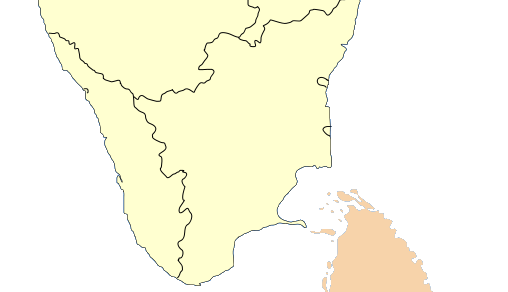
\includegraphics[width=\textwidth]{\imgpath/sourashtra.png}
 \caption[Sourashtra cities and towns]{Cities and towns having significant numbers of Sourashtra speakers  
\citep[following][3]{Ucida1979}. Ammapettai, listed by U\v{c}ida, is not indicated on the map as its reference is ambiguous (Ammapettai, Erode District; Ammapettai, Thanjavur district; or possibly Ammapet, a neighbourhood of Salem). It should also be noted that U\v{c}ida adds 'etc.' to his list of locations in Tamilnadu.
}
 \label{smith:fig:sourashtra}
\end{figure}


Sourashtra is a distant relative of Gujarati spoken by a traditionally weaving community in Tamil Nadu and adjacent areas of Andhra Pradesh, predominantly in cities such as Madurai and Tanjavur. According to their own traditions, the Sourashtra-speaking community left their home in what is modern Gujarat in the 11th century, and after stops in Marathi and Telugu-speaking regions probably started arriving in the Tamil country in the 16th C. Sourashtra continues as the exclusive home language in most households and is the first language of all Sourashtra speakers. Again, there is no documentation of the early sociolinguistic context, but as far as one can tell, Sourashtra has continuously been the spoken language of a sizeable community, and at no point has its transmission from one generation to the next been disrupted. Despite heavy Dravidianization \citep[e.g.][]{Pandit1972}, the language, like Sinhala, retains some Indo-Aryan derived morphology, including the remains of subject-verb agreement. The Sourashtra community spent extended periods among Marathi and Telugu speakers before coming into contact with Tamil and has many lexical items of Telugu and Marathi origin. Long periods of contact may well have left their mark on the grammar as well. Sourashtra has always been a minority language and there is no evidence that Tamils have ever spoken the language. Thus Dravidian influence in the language is due exclusively to Sourashtra speakers' bilingualism in Tamil/Telugu (L1 $<$ L2).

\subsection{Sri Lanka Portuguese}

Sri Lanka Portuguese was born from Portuguese colonization of the island's littoral region (1515-1658). Created largely by Tamil and Sinhala speakers who learned simplified Portuguese as a second language, it became the language of identity for the mixed-race community that was engendered by unions of local women and Portuguese men and their camp-followers. It throve during the subsequent period of Dutch rule (1656-58), but began a long decline after the British take-over in 1795. There remains a small (but unknown) number of speakers, and the language was on the verge of extinction even before the twin disasters of civil war and tsunami. See \citet{Nordhofffcslp} for a recent report. Nevertheless, the Dravidian features found in Sri Lanka Portuguese are \textit{not} due to language death -- most, if not all, were already in place by the mid 19\textsuperscript{th} C. (\citet[231-214]{Smith1979convergence},\citet{Smith2005missionnaires}). Sri Lanka Portuguese is uncontroversially a creole, arising at about the same time, and in the same socio-political context as its sister varieties of Indo-Portuguese, thus the Dravidian influence is attributable in the initial stages to the L1 of local learner/creators (L1 $>$ L2); once the community was established, influence could also flow in the reverse direction (L1 $<$ L2). 

There is evidence of ongoing substrate (acting as adstrate) influence on word order in Korlai Portuguese \citep{Clements1991}, and more general evidence that both lexifier and sub/adstrate exert an influence on an established creole \citep{Clements2009,Smithfc}. The ouster of the Portuguese from Sri Lanka by the Dutch by 1658 left free rein to the L1 $<$ L2 influence of the substrates as adstrates. For most of the structures of the language, it is unclear whether the source is Sinhala or Tamil \citep[216]{Smith1979convergence}; from a historical point of view, since the Portuguese first established themselves in the southwest, Sinhala-speaking, area of the island, it is likely that Sinhala was the most important early influence \citep[cf.][254-5]{Jayasuriya1999substratum}. Once the language had been spread to Tamil speaking areas, Tamil could been the source of both L1 $>$ L2 (particularly through intermarriage) and L1 $<$ L2 influence. However, the possibility must also be entertained that certain South Asian features were already present in the pidgin Portuguese/foreigner talk brought to Sri Lanka; such would seem to be the case for the postnominal genitive marker \textit{{}--su(a)}, found in Sri Lanka as well as in other Indo-Portuguese varieties. 

\subsection{Sri Lanka Malay}

\citet{SmithEtAl2006cll} give the following account of the origins of Sri Lanka Malay:

\begin{quote}
``SLM is spoken by descendants of immigrants from the Indonesian archipelago and the Malay peninsula brought to Sri Lanka by Dutch and British colonial administrations. Most of the immigrants were soldiers, with smaller numbers of political exiles, slaves, and convicts. {\dots}The first waves of immigrants brought to Sri Lanka by the Dutch colonial administration, beginning in 1656, came from various locations in the Indonesian archipelago, and were native speakers of a number of West Austronesian languages.'' \citep[2006:160-1]{SmithEtAl2006cll}
\end{quote}

This much is uncontroversial. Disagreement arises, however, over other statements:

\begin{quote}
``From their arrival, the immigrants closely associated with the established Tamil-speaking Sri Lanka ``Moor'' community, with whom they shared the Muslim religion \citep[45]{Hussainmiya1987}. As most of the immigrants were soldiers, and therefore single males for the most part, a high degree of intermarriage with the Moor community was inevitable. Through this interaction between the two communities, a new language arose, strongly influenced by Tamil structure, with a lexicon almost entirely derived from Malay.'' (2006:160)
\end{quote}

The claim that the Moors played a primary role in providing human and linguistic input to the new community and its language has been challenged, \citet{Ansaldo2008genesis} going so far as to claim that it reflects a ``Tamil bias''. At issue also is the question of whether there was a disruption in the transmission of Malay serious enough to warrant the application of the term ``creole''. On the other hand, some claim Sri Lanka Malay is a contact language of a different type: a mixed language \citep{Meakinstoappear}.

One important aspect of the contact situation that has largely been ignored is the presence of Standard Malay in the 19\textsuperscript{th} century, particularly through the provision of Malay-language education for Malay soldiers and their families. It is known that the presence of its lexifier and its availability through education exerts a significant influence on a creole. Therefore, it is quite likely that some Standard Malay features were introduced into Sri Lanka Malay during this century.

\section{Dravidian verbal noun}

The verbal noun is a well-established structure in several southern Dravidian languages \citep[See][155 for descriptive sources]{Gair1986}  which has spread to all four of the languages in contact with Tamil described here. 

\subsection{The Tamil verbal noun}

The verbal noun in Tamil is formed by adding a 3\textsuperscript{rd} person non-human singular pronoun to a tensed verbal stem. The Sri Lanka Tamil present and past verbal nouns for the verbs \textit{poo} `go' and \textit{kee{\textrtaill}} `hear; ask' are shown in \xref{smith:ex:5}. 

\ea\label{smith:ex:5} 
{}[Sri Lanka Tamil, constructed]
\ea
\gll poo-r-adu; poo-n-adu \\
go-\textsc{prs}-3\textsc{sg}.\textsc{nhum}; go-\textsc{past}-3\textsc{sg}.\textsc{nhum} \\
\ex
\gll kee-kk\footnotemark{}{}-r-adu; kee-{\textrtailt}{\textrtailt}-adu \\
hear-\textsc{aug}-\textsc{prs}-3\textsc{sg}.\textsc{nhum}; hear-\textsc{aug}-\textsc{past}-3\textsc{sg}.\textsc{nhum}\\
\z
\z
\footnotetext{{\em -kk-}
 is a stem augment found in the present stem and infinitive of certain verb classes.}

The stem to which the pronoun is affixed is arguably a verbal adjective (e.g. \textit{poo-r-a, poo-n-a, kee-kk-r-a, kee-{\textrtailt}{\textrtailt}-a}) which has undergone apocope, since this is the stem that combines with other pronouns, as in the Sri Lanka Tamil habitual shown in \xref{smith:ex:6} Apocope of the final vowel is seen in \xref{smith:ex:7} when the 3\textsuperscript{rd} person nonhuman pronoun is used; this form is homophonous with the verbal noun.

\ea\label{smith:ex:6} 
{}[Sri Lanka Tamil, elicited]
\gll naan tyuvishan-ukku poo-r-a-naan.\\
1\textsc{sg} tuition-\textsc{dat} go-\textsc{prs}-\textsc{adjz}-1\textsc{sg}\\
`I go for tuition.'
\z

\ea\label{smith:ex:7} 
{}[Sri Lanka Tamil, elicited]
\gll adu tyuvishan-ukku poo-r-{\O}-adu\\
3\textsc{sg}.\textsc{nhum} tuition-\textsc{dat} go-\textsc{prs}-\textsc{adjz}-3\textsc{sg}.\textsc{nhum}\\
`He/she [child] goes for tuition.'
\z

The functions of the verbal noun differ somewhat from one variety of Tamil to another. The principal varieties mentioned here are Sri Lanka Tamil (especially Jaffna Tamil), Shonam (Sri Lanka Muslim Tamil) and Indian Tamil (in which there is much regional and social variation). Although examples may be specified as one variety or another because of phonological, morphological or lexical specificities, usages are pan-dialectal unless otherwise specified.

\subsubsection{Nominal clause }%5.1.1
The verbal noun is used to nominalize a clause so that it may then function as the subject or complement of a verb, complement of a postposition etc. The verbal noun is the only signal of subordinate status; other elements of the clause remain the same as they would be in a main clause. This contrasts with languages like English in which a nominalized verb may take different kinds of arguments from its main clause counterpart. (For example, \textit{The hunters shot the lions.} vs. \textit{The shooting of the lions by the hunters.}) 

\ea\label{smith:ex:8}
{}[Shonam; elicited]
\gll sigarat ku{\textrtaild}i-kk-r-adu o{\textrtaild}ambu-kku nall=aa ille. \\
cigarette smoke-\textsc{aug}-\textsc{prs}-\textsc{nmlz} body-\textsc{dat} good=\textsc{advz} \textsc{neg}\\
`Cigarette smoking is not good for health.'
\z


\subsubsection{(Past) experiential negative}%5.1.2
The experiential negative is formed by adding the negative \textit{ille} to the past verbal noun.

\ea\label{smith:ex:9}
{}[Tamil: elicited]
\gll naan ange poo-n-ad ille. \\
1\textsc{sg} there go-\textsc{past}-\textsc{nmlz} \textsc{neg}\\
 `I never went there./I have never been there.'
\z

\subsubsection{(Present) habitual negative}%5.1.3
The habitual negative is formed by adding the negative \textit{ille} to the present verbal noun.

\ea\label{smith:ex:10}
{}[Tamil: elicited]
\gll naan ange poo-r-ad ille \\
1\textsc{sg} there go-\textsc{prs}-\textsc{nmlz} \textsc{neg} \\
 `I don't go there.'
\z

\ea\label{smith:ex:11}
{}[Tamil: elicited]
\gll naan sigarat ku{\textrtaild}ikk-r-ad ille \\
1\textsc{sg} cigarette smoke-\textsc{prs}-\textsc{nmlz} \textsc{neg} \\
 `I don't smoke.'
\z

\subsubsection{`Thinking of V-ing'}%5.1.4

In Indian Tamil, the equivalent of the English expression `thinking of V-ing' is rendered by present verbal noun with the addition of the adverbializer \textit{=aa} and the verb \textit{iru }`be'. This usage is not found in Sri Lankan Tamil varieties.

\ea\label{smith:ex:12}
{}[Indian Tamil: elicited]
\gll adan-aala sigara{\textrtailt} ku{\textrtaild}i-kk-r=adu vi{\textrtaild}-r-ad=aa iru-kk-r-een\\
That-ins cigarette smoke-\textsc{aug}-\textsc{prs}-\textsc{nmlz} leave-\textsc{prs}-\textsc{nmlz}=\textsc{advz} be-\textsc{aug}-\textsc{prs}-1\textsc{sg}\\
`Therefore I am thinking of giving up cigarette smoking.'
\z


\subsubsection{Focus/cleft (optional)}%5.1.5

A non-verbal constituent of a Tamil main clause may be focussed by the addition of the focus particle {\em =taan/daan}. The verb is optionally nominalized. If the verb is nominalized, the focal element may be placed in post-verbal position, where it carries the major final intonation contour. This contrasts with ``afterthought'' elements which follow a non-nominalized verb; in this case the major final intonation contour falls on the verb and the ``afterthought'' is on low pitch. \xref{smith:ex:12} shows an unfocussed sentence; \xref{smith:ex:13} shows various focussing options. Murugaiyan notes that when the verb is nominalized the focus marker is pragmatically obligatory   \citep[56]{Murugaiyan2009}.

\ea\label{smith:ex:12}
{}[Tamil, elicited]
\gll naan bas-le poo-n-een.\\
1\textsc{sg} bus-\textsc{loc} go-\textsc{past}-1\textsc{sg} \\
`I went by bus.'
\z


\ea\label{smith:ex:13}
{}[Tamil, elicited] 
\ea
\gll naan=taan bas-le poo-n-een. \~{} *bas-le poo-n-een naan=taan  \\
1\textsc{sg}=\textsc{foc} bus-\textsc{loc} go-\textsc{past}-1\textsc{sg} \\
\ex
\gll naan=taan bas-le poo-n-adu. \~{} bas-le poo-n-adu naan=taan.\\
1\textsc{sg}=\textsc{foc} bus-\textsc{loc} go-\textsc{past}-\textsc{nmlz} \~{} bus-\textsc{loc} go-\textsc{past}-1\textsc{sg} 1\textsc{sg}=\textsc{foc}\\
`I was the one who went by bus; \textit{I} went by bus; it was I who went by bus.'
\z
\z

Since WH-words are inherently focussed, they behave in the same way as a focussed element, viz. they can occur with a verb showing subject concord or with a nominalized verb and with the latter they may be postposed. These possibilities are illustrated in \xref{smith:ex:14} and \xref{smith:ex:15}. 

\ea\label{smith:ex:14}
{}[Tamil, elicited]
\ea
\gll yaar ange poo-n-anga? \~{} *ange poon-aanga yaar?\\
who there go-\textsc{past}-3\textsc{pl} \\
\ex
\gll yaar ange poo-n-adu? \~{} ange poo-n-adu yaar?\\
who there go-\textsc{past}-\textsc{nmlz} \~{} there go-\textsc{past}-\textsc{nmlz} who\\
`Who went there?'
\z
\z

\ea\label{smith:ex:15}
{}[Tamil, elicited]
\ea
\gll avan enge poo-n-aan? \~{} *avan poo-n-aan enge?\\
 3\textsc{sg}.\textsc{nhon} where go-\textsc{past}-3\textsc{sg}.\textsc{nhon} \\
\ex
\gll avan enge poo-n-adu? \~{} avan poo-n-ad enge?\\
3\textsc{sg}.\textsc{nhon} where go-\textsc{past}-\textsc{nmlz} \\
 `Where did he go?'
\z
\z

Speakers of both Indian and Sri Lanka Tamil have expressed unease with a nominalized verb when the subject is honorific, as in \xref{smith:ex:16}. This seems to be because of the use of the nonhuman pronoun as nominalization marker. 

\ea\label{smith:ex:16}
\ea
{}[Tamil, elicited]
\gll niinga enge poo-n-iinga? \\
2\textsc{hon} where go-\textsc{past}-2\textsc{hon}\\
\ex
\gll (*)niinga enge poo-n-adu? \\
 2\textsc{hon} where go-\textsc{past}-\textsc{nmlz} \\
`Where did you go?'
\z
\z

\subsubsection{Unspecified subject (optional)}%5.1.6
 When the subject of the main clause is unspecified (and unexpressed), the verb may be optionally nominalized. Often the most appropriate English rendering uses the passive voice. Again, the nominalized verb is dispreferred for some speakers when the nonhuman marking of the nominalized verb clashes with an honorific participant, as in \xref{smith:ex:19}.

\ea\label{smith:ex:17}
{}[Tamil, Sourashtra:07B\footnotemark{}]
\gll onga pa{\textrtaill}{\textrtaill}ikkuu{\textrtaild}att-ile ennam=oo na{\textrtaild}a-kk-r-adu\\
 2\textsc{hon}.\textsc{gen} school-\textsc{loc} what-\textsc{indef}  run-\textsc{aug}-\textsc{prs}-\textsc{nmlz} \\
 `They are putting something on in your school.'
\z
\footnotetext{ Tamil examples sourced from ``SourashtraXXS'' are from the Tamil translations of conversational conversations in Sourashtra recorded in Madurai in 1989-90; XX refers to the cassette no. and S is the side (A or B). Tamil translations were initially provided by bilingual Sourashtra speakers and were checked for naturalness by a Tamil speaker. All examples cited here have been checked with at least one additional Tamil speaker.}


\ea\label{smith:ex:18}
{}[Tamil, elicited]
\gll ad-e {\em cup}=nu solr-adu\\
that-\textsc{acc} cup=\textsc{quot} say-\textsc{prs}-\textsc{nmlz} \\
`That's called a ``cup''.'
\z

\ea\label{smith:ex:19}
{}[Indian Tamil; Sourashtra:05A]
\gll avanga{\textrtaill}-e {\em atte}=nu sollu-v-oom./(*)sol-r-adu\\
3\textsc{pl}-\textsc{acc} {\em atte}=\textsc{quot} say-\textsc{fut}-1\textsc{pl}/say-\textsc{prs}-\textsc{nmlz} \\
`They are called ``atte'' [=father's mother].'
\z

\subsubsection{Main Clause with future ref: (IT only, dialectal?, optional)}%5.1.7

In a main clause with future time reference a present nominalized verb may sometimes be used in place of a future-tensed verb with subject agreement. This usage is not reported in the literature and has not been investigated in detail. It is not found in Sri Lanka and may be geographically restricted within India. 

\ea\label{smith:ex:20}
{}[Indian Tamil, Sourashtra:05A]
\gll id ellaam diipaava{\textrtaill}i ka{\textrtaill}i-nj-a peragu gavani-pp-aanga/gavani-kk-r-adu\\
3\textsc{sg}.\textsc{nhum} all Divali finish-\textsc{past}-\textsc{adjz} after look.after-\textsc{fut}-3\textsc{pl}/look.after-\textsc{aug}-\textsc{prs}-\textsc{nmlz} \\
`[They] will look after all this when Divali is over.'
\z


\subsection{Sinhala `focus' form}


The Sinhala focus (or `emphatic') form is constructed by adding \textit{ee} to a tensed (prs or pst) stem, as seen in \xref{smith:ex:21} for \textit{bala-n-awaa/} \textit{b{\ae}luw-aa }`see-\textsc{prs}-fin/see.\textsc{past}-fin'.\footnote{It is not the general scholarly practice to decompose Sinhala verbs into concatenative morphemes. I do so here only to make clear the structure of the focus form. Some problems associated with the analysis here are as follows. First, the fact that \textit{bala} by virtue of its opposition to \textit{b{\ae}luw} also indexes nonpast is not indicated. Second, the single \textit{--}\textit{n- }found in the present form also indexes ``finite'', since the present focus form and the infinitive have \textit{--}\textit{nn-}. Third, ``finite'' is an unsatisfactory label; perhaps ``unmarked'' would be better. Finally, the ``finite'' affixes, by virtue of their difference, also index tense.
}
The origin of this form seems to be a verbal adjective to which is added a 3\textsc{sg}.m/n suffix (\citet[156]{Gair1986}, citing \citet[134-5]{Geiger1938}; i.e. it is a calque on the Tamil model. This analysis is now opaque, and as Gair points out, the form is ``not a clearly nominal form at present'' (1998:156). 
Indeed, Sinhala has two synchronic nominalization strategies (e.g.\textit{ balaa-ma, balana-eka} `seeing', the latter a more recent calque on Tamil\footnote{An anonymous reviewer points out a third form, b{\ae}li-lla.})), which are used for non-\textsc{foc}us nominalizations, e.g., the nominalized verb in \xref{smith:ex:22} The focus form is tightly integrated into the grammar of Sinhala; its functions are outlined below. For a detailed description, see \citet{Gair1986}.

\ea\label{smith:ex:21}
{}[Sinhala: elicited]
\gll bala-nn-e; b{\ae}luw-ee\\
see-\textsc{prs}-\textsc{foc}; see.\textsc{past}-\textsc{foc}\\
\z

\ea\label{smith:ex:22}
{}[Sinhala: elicited]
\gll sigara{\textrtailt} bii-ma saukya-{\textrtailt}a ho\textsuperscript{n}da n{\ae}{\ae}\\
cigarette smoke-\textsc{nmlz} health-\textsc{dat} good \textsc{neg}\\
`Cigarette smoking is not good for the health.'
\z


\subsubsection{Focus constructions (obligatory)}%5.2.1
In contrast to Tamil, where the nominalized verb is optional in focus constructions, in Sinhala the focus form is obligatory whether or not the focal element is postposed. \xref{smith:ex:23} gives a non-\textsc{foc}us construction and \xref{smith:ex:24} its focussed equivalents. 

\ea\label{smith:ex:23}
{}[Sinhala: elicited]
\gll mama bss-ek-ee giyaa\\
1\textsc{sg} bus-\textsc{sg}.\textsc{def}-\textsc{loc} go.\textsc{past}\\
`I went by bus.'
\z


\ea\label{smith:ex:24} 
{}[Sinhala, elicited]
\ea
\gll mama=y bas-ek-ee giy-ee/*giyaa \\
1\textsc{sg}=\textsc{foc} bus-\textsc{sg}.\textsc{def}-\textsc{loc} go.\textsc{past}-\textsc{foc}/*go.\textsc{past}\\
\ex
\gll   b{\textschwa}s-ekee giy-ee(/*giyaa) mama=y \\
     bus-\textsc{def}.\textsc{loc} go.\textsc{past}-\textsc{foc}/*go.\textsc{past} 1\textsc{sg}=\textsc{foc}   \\
`I was the one who went by bus.'
\z
\z


As expected, the focus form is also obligatory in WH-questions, as seen in \xref{smith:ex:25}. Unfocussed polar questions, on the other hand, use the `finite' form, as seen in \xref{smith:ex:26}.

\ea\label{smith:ex:25}
{}[Sinhala, elicited]
\gll oyaa kohee=da giy-ee?/*giyaa \~{} oyaa giy-ee(/*giyaa) kohee=da?\\
2\textsc{sg} where=\textsc{interr} go.\textsc{past}-\textsc{foc}/*go.\textsc{past}\\
`Where did you go?'
\z

\ea\label{smith:ex:26}
\gll oyaa kola{\umb}a  giyaa=da?\\
2\textsc{sg} Colombo go.\textsc{past}=\textsc{interr}\\
`Did you go to Colombo?'
\z

\subsubsection{Negation (obligatory)}%5.2.1
In 5.1.2 and 5.1.3 we saw that the Tamil verbal noun combines with the negative marker to render specialized negative meanings (viz. experiential and habitual). In Sinhala, by contrast, \textit{all} negative sentences require the focus form. \xref{smith:ex:27} shows a positive sentence and \xref{smith:ex:28} its negative counterpart

\ea\label{smith:ex:27}
{}[Sinhala; elicited]
\gll mama kola{\umb}a yanawaa/giyaa\\
1\textsc{sg} Colombo go.\textsc{prs}/go.\textsc{past}\\
`I'm going to Colombo / I went to Colombo'
\z

\ea\label{smith:ex:28}
{}[Sinhala; elicited]
\ea
\gll mama kola{\umb}a yann-ee n{\ae}{\ae}\\
1\textsc{sg} Colombo go.\textsc{prs}-\textsc{foc} \textsc{neg}\\
`I'm not going to Colombo; I didn't go to Colombo.'
\ex
 mama kola{\umb}a giy-ee n{\ae}{\ae}\\
 1\textsc{sg} Colombo go.\textsc{past}-\textsc{foc}\\
\ex *mama kola{\umb}a giyaa/yan{\textschwa}waa n{\ae}{\ae}

 1\textsc{sg} Colombo go.\textsc{past}/go.\textsc{prs} \textsc{neg} \\
\z
\z

\subsection{Sourashtra \textit{{}-atte/-eyo} }

Sourashtra forms verbal nouns by adding --\textit{atte} (present) and --\textit{eyo} (past) to a verb base, as illustrated for three verbs in \xref{smith:ex:29}; neither form is found in Gujarati. The present form originates from an Indo-Aryan imperfective participle in --\textit{at} ($<$OIA \textit{{}--anta}) plus a 3\textsc{sg} pronoun \textit{te }(\citet[272]{Masica1991}, \citet[93,100]{Cardona1965}; the past form is from an Indo-Aryan perfective participle in \textit{{}--ey} ($<$OIA --\textit{ita}) plus a m.sg. marker -\textit{o }(\citet[272]{Masica1991}, \citet[100-1]{Cardona1965}. Both formations are now opaque. The functions of Sourashtra\textit{ --atte/-eyo} are outlined below.

\ea\label{smith:ex:29}
\ea
\gll ker-atte/ker-eyo \\
do-\textsc{prs}.\textsc{nmlz}/do-\textsc{past}.\textsc{nmlz} \\
\ex sig-atte/sig-eyo \\
 learn-\textsc{prs}.\textsc{nmlz}/learn-\textsc{past}.\textsc{nmlz}
\ex men-atte/men-eyo\\
say-\textsc{prs}.\textsc{nmlz}/say-\textsc{past}.\textsc{nmlz}\\
\z
\z

\subsubsection{Nominalized clause}%5.3.1

This function closely parallels the corresponding Tamil function (5.1.1).

\ea\label{smith:ex:30}
{}[Sourashtra:05A\footnotemark{}]
\gll tunko puus men-atte pus-unaan\\
2\textsc{hon}.\textsc{dat} listen.\textsc{imp} say-\textsc{prs}.\textsc{nmlz} listen-\textsc{fut}.\textsc{neg}.\textsc{pl}\\
`You won't listen to what anyone tells you.' 
(Lit: You won't listen to [someone] saying ``listen!'')
\z
% \footnotetext{ For an explanation of Sourashtra:XXS, see footnote 4.}


\ea\label{smith:ex:31}
{}[Sourashtra:29A]
\gll avro gaamu thov-eyo konni serkko cal-ani\\
1\textsc{pl}.\textsc{gen} town put-\textsc{past}.\textsc{nmlz} nothing well go-\textsc{neg}\\
`What they set up in our town [i.e. the community association] did not go well at all.'
\z


\subsubsection{Focus (optional)}%5.3.2

As in Tamil the use of nominalization in focused sentences is optional. (See \xref{smith:ex:36} for a non-nominalized example.) The focussed nominal may be postposed, and the construction is commonly used with WH-interrogatives.

\ea\label{smith:ex:32}
{}[Sourashtra:05A]
\gll atto soo mha{\textrtaild}a munda{\textrtaild}ii=nnaa kha{\textrtaild}-eyo\\
now six month before=\textsc{foc}.\textsc{tag} buy-\textsc{past}.\textsc{nmlz}\\
`Now it was six months ago that they bought it, eh.'
\z

\ea\label{smith:ex:33}
{}[Sourashtra:05A]
\gll teno tee{\textrtaild}uu=s jiy-eyo\\
3\textsc{sg}.C there=\textsc{foc} go.\textsc{past}-\textsc{past}.\textsc{nmlz}\\
`It was there that he went.'
\z

\ea\label{smith:ex:34}
{}[Sourashtra:34A]
\gll jeendipuramu jaa-riyo basu koo{\textrtailt} hing-atte?\\
Jeendipuram go-\textsc{adjz} bus where get.on-\textsc{prs}.\textsc{nmlz}\\
`Where do you get on the bus that goes to Jeendipuram?'
\z

\ea\label{smith:ex:35}
{}[Sourashtra:35A]
\gll tumi me{\textrtaild}raasu-m uj-eyo koo{\textrtailt}? \\
2\textsc{hon} Madras-\textsc{loc} be.born-\textsc{past}.\textsc{nmlz} where\\
`Where in Madras were you born?'
\z

\ea\label{smith:ex:36}
{}[Sourashtra:35A]
\gll hindo koo{\textrtailt} jiy-aasi, tumi?\\ 
today where go.\textsc{past}-\textsc{past}.\textsc{pl} 2\textsc{hon} \\
 `Where did you go today?'
\z


\subsubsection{Habitual negative }%5.3.3
As in Tamil, the present verbal noun combines with a negative marker to encode habitual negative. The experiential negative uses an alternate formation for the past verbal noun using the suffix \textit{{}--iriyo, }as seen in \xref{smith:ex:38}.

\ea\label{smith:ex:37}
{}[Sourashtra:34A]
\gll tellamaam puuraa-k ami ja-atte nhaa \\
that.\textsc{loc} all-\textsc{dat} 2\textsc{pl} go.\textsc{prs}-\textsc{prs}.\textsc{nmlz} \textsc{neg} \\
`We don't go there and all.'
\z

\ea\label{smith:ex:38}
{}[Sourashtra, elicited]
\gll teno ji-iriyo nhii\\
3\textsc{sg} go.\textsc{past}-\textsc{past}.\textsc{nmlz} \textsc{neg}\\
`He never went/He hasn't gone (ever)'
\z

\subsubsection{Unspecified subject: (optional) }%5.3.4

As in Tamil, a nominalized verb may be used with an unspecified subject, often as a passive equivalent. Unlike Tamil, Sourashtra has no restriction on using the verbal noun with an honorific participant, as in \xref{smith:ex:40}. This may be because the nominalizing suffixes are not synchronically linked with non-human forms as are the corresponding Tamil suffixes.

\ea\label{smith:ex:39}
{}[Sourashtra:07B]
\gll ture po{\textrtaill}{\textrtailt}am-u kaay=ki dham-atte\\
  2\textsc{hon}.\textsc{gen} school-\textsc{loc} what=\textsc{indef} run-\textsc{nmlz} \\
`They are putting something on in your school.'
\z

\ea\label{smith:ex:40}
{}[Sourashtra:05A]
\gll tenko `ph\~oy' men-atte\\
3\textsc{pl}.\textsc{acc} `ph\~oy' say-\textsc{prs}.\textsc{nmlz}\\
`They are called ``ph\~oy'' [father's brother].'
\z

\subsubsection{Main Clause with future reference (optional) }%5.3.5

As in Tamil, a main clause with future reference may have a verbal noun instead of an agreement-inflected verb. Sourashtra uses this formation more frequently than Tamil.

\ea\label{smith:ex:41}
{}[Sourashtra:05A]
\gll ella aski diva{\textrtaill}i ser-et-teer gavunc-atte\\
this all Divali finish-\textsc{past}.\textsc{adjz}r-after look.after-\textsc{prs}.mnlz\\
`[They] will look after all this when Divali is over.'
\z


\subsubsection{Relative clause (variant)}%5.3.6

\citet{Pandit1972}, in his pioneering work on Sourashtra pointed out that its relative clause structures were similar to Tamil rather than to Gujarati. The salient characteristics of this Dravidian-style structure are prenominal position, absence of a relative pronoun and dependent verb form (the verbal adjective) that marks tense but not agreement. Sourashtra has two forms for the present verbal adjective, one in \textit{{}--atte, }seen in \xref{smith:ex:42}, the other in \textit{\-ariyo}, seen in \xref{smith:ex:43}\textit{. }Neither of these is used exclusively as a dependent form: \-\textit{{}-atte }is familiar as our present verbal noun; \-\textit{{}-ariyo} forms a main verb unmarked for agreement and is also an alternative (but rarer) verbal noun formation. As verbal adjectives, the two forms are almost in complementation, with \textit{{}-ariyo} in general use before a noun head. As in Tamil, Sourashtra relative clauses can modify pronouns and time nominals which contract with the verbal adjective. In Sourashtra the present verbal adjective used in these combinations is almost exclusively the\textit{ -atte }form (contracted to \textit{{}--at} before following \textit{te-)}. The complementation is spoilt, however, by the occasional occurrence of \-\textit{{}--atte} with noun heads as in \xref{smith:ex:42} and of \-\textit{{}--ariyo} with a pronoun head. 

The past verbal adjective is formed with \-\textit{{}--e (-et }before \textit{te-)} as seen in \xref{smith:ex:41} above. The past verbal noun in \--\textit{eyo} never marks a relative clause.

\ea\label{smith:ex:42}
{}[Sourashtra:05A]
\gll macc-i        phil-l-atte savlo pay-et kha{\textrtailt}-{\textrtailt}-uvaay\\
change-\textsc{cp} wear-\textsc{ben}-\textsc{prs.nmlz} sari want-\textsc{cond} buy-\textsc{pfv}-\textsc{per}\\
`If [you] want a house sari [we] can buy [one]' (Lit: `a sari that [you] wear having changed')
\z

\ea\label{smith:ex:43}
{}[Sourashtra:05A]
\gll telle phalaar hand-i vikk-ariyo {\textscriptg}heer le{\textscriptg}utto kyaa?\\
that idli prepare-\textsc{cp} sell-\textsc{prs}.\textsc{nmlz} house near \textsc{interr}\\
`Near that house where [they] prepare and sell idli?'
\z

\ea\label{smith:ex:44}
{}[Sourashtra:07B]
\gll dekk-et-tenko puuraa bovd-ariyo; av-at-tenu av-an\\
see-\textsc{past}.\textsc{adjz}-3\textsc{pl}.\textsc{acc} all invite-\textsc{nmlz}; come-\textsc{prs}.\textsc{nmlz}-3\textsc{pl} come-\textsc{fut}.\textsc{p}\\
`We'll invite all those whom we saw. Those who come will come.'
\z

\subsection{Sri Lanka Portuguese \textit{ki-}}

Sri Lanka Portuguese forms its nominalized verb with the verbal prefix \textit{ki-}, followed optionally by the tense markers \textit{ta-}(\textsc{prs}) or \textit{jaa-}(\textsc{past}) as illustrated in \xref{smith:ex:45} for \textit{faya} `do'.

form: ki+(TNS)+Verb base. 

\ea\label{smith:ex:45}
{}[Sri Lanka Portuguese, constructed]
\gll ki-faya / ki-ta-faya / ki-jaa-faya \\
\textsc{nmlz}-do / \textsc{nmlz}-\textsc{prs}-do / \textsc{nmlz}-\textsc{past}-do\\
\z

The marker \textit{ki-} derives from the Ptg. relative clause marker \textit{que, }particularly in cleft constructions of the type\textit{ }illustrated in \xref{smith:ex:46}, for which the corresponding Sri Lanka Portuguese sentence is given in \xref{smith:ex:47}. 

\ea\label{smith:ex:46}
{}[Portuguese, elicited]
\gll (\'E) eli que foi l\'a\\
be.3\textsc{sg} 3\textsc{sg}.\textsc{masc} \textsc{rel} go.\textsc{past}.3\textsc{sg} there\\
`It was he who went there.'
\z

\ea\label{smith:ex:47}
{}[Sri Lanka Portuguese, constructed]
\gll eli mee ala ki-jaa-foi\\
3\textsc{sg} \textsc{foc} there \textsc{nmlz}-\textsc{past}-go\\
\z

The functions of \textit{ki- }are outlined in the following subsections. Verbs may also be nominalized by use of the suffix \textit{{}--saam, }as in \textit{midi-saam} `measurement' from \textit{midii }`measure', illustrated in \xref{smith:ex:48}, or \textit{arnaga-saam} `hatred; cursing' from \textit{arnagaa} `curse'. This formation does not participate in any of the constructions outlined below, however. It is best treated as a lexical derivation, which does not always produce fully predictable meanings. 

\ea\label{smith:ex:48}
{}[Sri Lanka Portuguese, conversational, Field notes:2235\footnotemark{}]
\gll t{\textopeno}{\textopeno}na aka midi-saam inda u{\ng}a pa-araa naa-pooy=ski\\
later that measure-\textsc{nmlz} yet one \textsc{inf}-escape \textsc{fut}.\textsc{neg}=\textsc{hbl}=\textsc{rep}\\
`Afterwards, someone else cannot ignore that [official] measurement, apparently.'
\z
\footnotetext{ Numbers refer to the item in the author's Sri Lanka Portuguese field notes, 1974-5. Examples taken from spontaneous recorded conversations among native speakers are marked `conversational'; examples spoken to the author without elicitation are marked `spontaneous'.}


\subsubsection{Relative clause (optional)}%5.4.1

Given its origin, it is not surprising to find that \textit{ki- }is used to mark a relative clause, as illustrated in \xref{smith:ex:49}. It is always optional and very rare in actual speech. All relative clauses directly precede the noun they modify, as in the other languages of the area. When \textit{ki- }is absent, there is no formal distinction between the verb of a relative clause and a main verb. 

\ea\label{smith:ex:49}
{}[Sri Lanka Portuguese, conversational, Field notes:5313] 
\gll nosa yuunyan-ntu (ki-)ti{\textltailn}a meshiin-su shatlk{\textepsilon}riya jaa-kaa-kebraa, um padaas\\
1\textsc{pl}.\textsc{gen} union-\textsc{loc} \textsc{nmlz}-be.\textsc{past} machine-\textsc{gen} shuttle.carrier \textsc{past}-\textsc{pfv}-break one piece\\
`A piece broke off the shuttle carrier of the machine that was in our union. 
\z
 
\subsubsection{Nominalized clause}%5.4.2

One of the most common uses of \textit{ki-} is to mark a nominalized clause. The usage parallels that of Tamil (5.1.1).

\ea\label{smith:ex:50}
{}[Sri Lanka Portuguese, conversational, Field notes:5173]
\gll tyuvishan ki-(ta)-daa graandi viraadu\\
tuition \textsc{nmlz}-\textsc{prs}-give big error\\
`Giving tuition is a great error.'
\z

\ea\label{smith:ex:51}
{}[Sri Lanka Portuguese, conversational, Field notes:5251]
\gll avara maara b{\textopeno}{\textopeno}rda ki-t-andaa kum, pa{\textrtaild}am-pa ki-t-andaa kum, kastiiv\\ 
now sea beside \textsc{nmlz}-\textsc{prs}-go and movie-\textsc{dat} \textsc{nmlz}-\textsc{prs}-go and trouble \\
`Now, going to the beach and going for a movie is troublesome.' [Context: speaking of decorous conduct for teen-aged girls.]
\z

\ea\label{smith:ex:52}
{}[Sri Lanka Portuguese, conversational, Field notes:1429]
\gll avara botus-pa ki-jaa-daa teem, aka graandi u{\ng} kaavs!\\
now 2\textsc{hon}-\textsc{dat} \textsc{nmlz}-\textsc{past}-give \textsc{pfv} that big one thing \\
`Now the fact that they have given [it] to you, that is a big thing!'
\z


\subsubsection{Focus construction (optional)}%5.4.3
As in Tamil, the use of the nominalized verb is optional in focus constructions. The focused element may optionally follow the verb, whether the verb is nominalized or not. This differs slightly from Tamil which only allows a post-verbal focus when the verb is nominalized. Example \xref{smith:ex:55} illustrates a post-verbal focus without nominalization of the verb.

\ea\label{smith:ex:53}
{}[Sri Lanka Portuguese, conversational, Field notes:4883]
\gll kii avara-su paav-su faartus-su pr{\textepsilon}{\textepsilon}su v{\textopeno}{\textopeno}nda pruveetu ki-ta-vii muytu m{\textepsilon}{\textepsilon}nis\\
what now-\textsc{gen} wood-\textsc{gen} thing.\textsc{pl}-gen price by profit \textsc{nmlz}-\textsc{prs}-come very less\\
`What! due to the price of timber products, the income comes to very little.'\footnotemark{}
\z
\footnotetext{ A putative alternative reading `the income which comes is very little' is ruled out by the fact that relative clauses are invariably prenominal in Sri Lanka Portuguese. }

\ea\label{smith:ex:54}
{}[Sri Lanka Portuguese, conversational, Field notes:2241]
\gll seem, midii-pa dispoos mee ki-poy sartifay=ski\\
yes measure-\textsc{dat} after \textsc{foc} \textsc{nmlz}=\textsc{hbl} certify=\textsc{rep}\\
`Yes, it is only after measuring [it] that [he] can certify [it], apparently.
\z


\ea\label{smith:ex:55}
{}[Sri Lanka Portuguese, conversational, Field notes:5111]
\gll alaa menaa bibeer=ley ti{\textltailn}a, jaa-paraa sudu akii mee; isti po{\textrtaild}iyaas jaa-nasa sudu akii mee\\
there of.course livelihood=\textsc{advz} be.\textsc{past}; \textsc{past}-live all here \textsc{foc} this child \textsc{past}-be.born all here foc\\
`We were there of course for employment [but] where we all lived was right here; where the children were born was right here.'
\z

\subsubsection{WH-Questions (optional)}%5.4.4
As in Tamil, WH-questions often have a nominalized verb, but do not require one, as \xref{smith:ex:58} shows. In all the examples in the corpus the WH-word occurs before, rather than after the verb. This may be a deficiency in the corpus or a difference with Tamil, which allows post-verbal WH-words.

\ea\label{smith:ex:56}
{}[Sri Lanka Portuguese, conversational, Field notes:5502]
\gll {\textopeno}kal{\textopeno}{\textopeno}ra isti-ntu doos taya daa senaa. sufraa see kii ki-faya? \\
then this-\textsc{loc} two tire give then swell \textsc{cond} what \textsc{nmlz}-do\\
`Put two tyres on this, then. If they blow out, what to do?'
\z

\ea\label{smith:ex:57}
{}[Sri Lanka Portuguese, conversational, Field notes:2282]
\gll eli oondi ki-t-andaa, akii benkal laraa-tu?\\
3\textsc{sg}.\textsc{nhon} where \textsc{nmlz}-\textsc{prs}-go here workshop leave-cp\\
`Where is he going, leaving his workshop here?'
\z

\ea\label{smith:ex:58}
{}[Sri Lanka Portuguese, song lyric, Field notes:5567]
\gll liimpu bistiidu buniitu, oondi boos t-andaa?\\
clean clothes pretty where 2\textsc{sg} \textsc{prs}-go\\
Where are you going, all dressed-up and pretty?
\z

\subsubsection{Habitual negative }%5.4.5
As in Tamil the nominalized verb participates in a habitual negative construction, seen here in \xref{smith:ex:59}.
                                            
\ea\label{smith:ex:59}
{}[Sri Lanka Portuguese, conversational, Field notes:4839]
\gll eev un t{\textepsilon}{\textepsilon}mpu taam ki-nuku-kuma, farii{\textltailn}a; aka diiya jaa-kuma-tu jaa-padiisa\\
1\textsc{sg} one time even \textsc{nmlz}-\textsc{neg}-eat, flour; that day \textsc{past}-eat-cp \textsc{past}-suffer\\
`I never ``used to''\footnotemark{} eat it, flour; one day I ate it and suffered.'
\z
\footnotetext{ In Sri Lankan English, as in other Asian varieties such as Singapore English, \textit{used to} can be used to signal present habitual.}



\subsubsection{Habitual}%5.4.6
In the first clause of the previous example the nominalized verb signals habitual. Further examples are seen below. Recall that Sri Lanka Tamil has evolved a habitual formation consisting of the verbal adjective followed by a pronoun agreeing with the subject (section 5.1, where the similarities between this formation and the verbal noun were pointed out). Since Sri Lanka Portuguese verbs do not exhibit agreement, its use of the verbal noun is thus inspired by the [Sri Lanka] Tamil construction. 

\ea\label{smith:ex:60}
{}[Sri Lanka Portuguese, spontaneous, Field notes:1151]
\gll botus-su kaaza-ntu verduura-s ki-simi{\textltailn}aa gardaa? \\
2\textsc{hon}-\textsc{gen} house-\textsc{loc} vegetable-\textsc{pl} \textsc{nmlz}-plant ben?\\
`Do you plant vegetables (for yourselves) at home?'
\z

\ea\label{smith:ex:61}
{}[Sri Lanka Portuguese, conversational, Field notes:5248]
\gll isti=ley greeya t-andaa kum ki-ta-vii mee\\
this=like church \textsc{prs}-go and \textsc{nmlz}-\textsc{prs}-come \textsc{foc}\\
`Like this, we go to church and come only.' (I.e. `We only go to and from church.')
\z


\subsection{Sri Lanka Malay \textit{yang-}}

Sri Lanka Malay forms nominalized verbs with the preverbal particle \textit{yang} (often reduced to [{\textltailn}{\textschwa}], [ayn] etc. ). The formation is illustrated in \xref{smith:ex:62} for \textit{maakan }`eat' and \textit{pii} `go'. 

\ea\label{smith:ex:62}
\gll yang-maakan; yang-pii\\
\textsc{nmlz}-eat; \textsc{nmlz}-go\\
\z

The language also retains the Malay nominalizing formation pref-V-\textit{an}, as in \textit{p{\textschwa}-cari-yan} `work'(N) from \textit{caari} `work'(V) and \textit{(k{\textschwa}-)susah-an} `sorrow' from \textit{suusa} `be sad'. This is primarily a lexical derivation and yields meanings that are not fully predictable.

The morpheme \textit{yang} derives from the Malay marker \textit{yang} which has a variety of, primarily pragmatic rather than strictly grammatical, functions, which it will be useful to survey before we examine the Sri Lanka Malay data. Englebretson demonstrates that in colloquial Indonesian \textit{yang} marks ``a continuum with three general foci{\dots} subordinate clauses modifying a head noun, phrasal constituents expressing presupposed information in clefts, and referring expressions serving as direct arguments of predicates or as unattached NPs''  \citep[24]{Englebretson2008}. The relative clause is illustrated in \xref{smith:ex:63}, where the clause introduced by \textit{yan g}modifies the head noun \textit{hal }`things'. A phrasal cleft is seen in \xref{smith:ex:64}, where \textit{yang baca gitu/yang baca itu} express presupposed, backgrounded information as opposed to the cleft focus \textit{dia}. In \xref{smith:ex:65} \textit{yang} marks the referring nominal expressions \textit{yang di kita, yang di dia}, and \textit{yang emas}; which contain no verbal element. 

\ea\label{smith:ex:63}
{}[Colloquial Indonesian, \citet[9]{Englebretson2008}, morp-by-morph glosses ammended for conformity]
\gll Masih ada hal yang perlu kita lakukan lagi\\
still be thing \textsc{yang} need 1\textsc{pl} do.\textsc{appl} again\\
`There are still things we need to do yet.' 
\z


\ea\label{smith:ex:64}
{}[Colloquial Indonesian, \citet[13-14]{Englebretson2008}]
\gll Maksudnya, dia yang baca gitu. Ayatnya dikasih Ari, dia yang baca itu\\
mean.\textsc{def} 3\textsc{sg} \textsc{yang} read thus verse.\textsc{def} \textsc{p}.give Ari 3\textsc{sg} \textsc{yang} read that\\
`So you mean it was she who read. You (Ari) gave her the verse and it was she who read it.'
\z

\ea\label{smith:ex:65}
{}[Colloquial Indonesian, \citet[16]{Englebretson2008}, morp-by-morph glosses amended for conformity]
\gll Yang di kita itu batu. Yang di dia itu yang emas\\
\textsc{yang} at 1\textsc{pl} that stone \textsc{yang} at 3\textsc{sg} that yang gold\\
`The one we've got is stone. The one he's got is the gold one.'
\z

Steinhauer's description of the core semantics of \textit{yang } again highlights its pragmatic functions: 

\begin{quote}
``\textit{yang} instructs the hearer to arrive at a projection in his mind of the thing meant through at least two stages: (1) a projection of the set of appropriate referents of the overt or implied antecedent, and (2) a projection of that subset which also belongs to the set of appropriate referents of the adjunct. In other words, \textit{yang} triggers the search for an antecedent and subsequently for a specified subset of the set of appropriate referents of this antecedent.'' (\citet[430-1]{Steinhauer1992}, cited by \citet[1987]{vanMinde2008})
\end{quote}

Van Minde, surveying older and regional material, notes additional discourse functions not usually reported in standard accounts of \textit{yang} that rely on material from standardized Bahasa Malaysia and Bahasa Indonesia. These are illustrated below. 

In \xref{smith:ex:66} \textit{yang }marks the theme/topic of the second and third sentences.

\ea\label{smith:ex:66}
{}[Malay, 1870, \citep[1994-5]{vanMinde2008}, morph-by-morph gloss supplied]
\gll Maka kalau boleh paduka sahabat sahaya beri sedikit surat kepada tuan dokter yang minta sedikit obat demam serta obat cacing barang enam bungkus. Yang obat demam sahaya makan sendiri yang obat cacing hendak memberi anak2 kecil \\
\textsc{cnj} \textsc{cond} can excellency friend 1\textsc{sg} give a.little letter to Mr. doctor \textit{yang} ask a.little medicine fever as.well.as medicine worm approximately six pack. \textit{yang} medicine fever 1\textsc{sg} eat \textsc{refl} \textit{yang} medicine worm intend \textsc{tr}.give child.\textsc{pl} small\\
`Could you please give me a note for the doctor asking for some medicine to suppress the fever and about six packets of medicine for worms. The fever medicine I will take myself, the vermifuge I will give to the children.'
\z

In \xref{smith:ex:67} \textit{yang} marks the clausal complement of \textit{meluluskan.} Van Minde remarks that in the dialectal folk stories collected in \citet{Toer1982} \textit{yang}, rather than standard \textit{bahwa, }is the usual clausal complementizer following verbs of speaking and cognition, adjectives and nouns (2008:1995-6).

\ea\label{smith:ex:67}
{}[Malay, 19\textsuperscript{th} C., \citet[1992]{vanMinde2008}, morph-by-morph gloss supplied]
\gll Maka adat itu meluluskan yang boleh sahaya menegurkan kelakuan raja\~{}raja yang tiada berpatutan, dengan tiada kena hukum bunuh atau rampas adanya \\ 
\textsc{cnj} law that permit \textit{yang} can 1\textsc{sg} criticize behaviour king\~{}\textsc{pl} \textit{yang} \textsc{neg} propriety, \textsc{cnj} \textsc{neg} pass punsihment kill or plunder being\\
`The laws allow that I criticize the unseemly behaviour of the rajas [corrected from raja's --IS] who kill and rob without being punished.'
\z

Finally, van Minde notes that in the pre-20\textsuperscript{th} century texts he surveyed, \textit{yang} is often omitted where the modern standard varieties would require it for complex attributes within an NP (such as relative clauses). He finds the same tendency in a modern Indonesian writer, Seno Gumira Ajidarma, whose ``language is quite direct, down-to-earth, with a strong admixture of spoken style language, while influence of Javanese and Jakarta Malay is also clearly felt.'' (2008:1997).

In contrast to its morphosyntactic fluidity in Malay/Indonesian, y\textit{ang }in Sri Lanka Malay is only pre-verbal marker. The closest pragmatic overlap between Malay/Indonesian and Sri Lanka Malay usages is found in cleft/focus constructions, as illustrated in \xref{smith:ex:64} above \xref{smith:ex:68} and \xref{smith:ex:69} below; see also 5.5.2. The functions of \textit{yang} in Sri Lanka Malay are surveyed in the following sections.

\ea\label{smith:ex:68}
{}[Malay, constructed]
\gll Saya yang pergi sana.\\
1\textsc{sg} \textit{yang} go there\\
`It was I who went there.'
\z

\ea\label{smith:ex:69}
{}[Sri Lanka Malay, elicited]
\gll se=jo saana yang-pii. \\
1\textsc{sg}=\textsc{foc} there \textsc{nmlz}-go\\
`It was I who went there.'
\z

\subsubsection{Relative clause (optional -- past only)}%5.5.1

\textit{Yang} retains its function as a relative clause marker, but its usage has become restricted to clauses with past reference where it replaces the past marker \textit{su-} \citep[For further details, see][]{BourdinEtAl2010}. \xref{smith:ex:70} illustrates this restriction. The standard Dravidian relative clause formation has the widest distribution in Sri Lanka Malay. Because of the obligatory replacement of the past-marker \textit{su- }by \textit{yang, }a past relative clause is distinguished from a past main clause. In the present and future, however, there is no formal distinction between the two.

\ea\label{smith:ex:70}
{}[Sri Lanka Malay, \citet[2-3]{BourdinEtAl2010};\footnotemark{} elicited]
\ea
\gll se yang-b{\textschwa}li kar merah\\ 
1\textsc{sg} \textsc{nmlz}-buy car red\\
`The car I bought is red.'
\ex
\gll *se (yang-)su-b{\textschwa}li kar merah\\
1\textsc{sg} \textsc{nmlz}-\textsc{past}-buy car red\\
`The car I bought is red.'
\ex
\gll se (*yang-)anti-b{\textschwa}li kar merah\\
1\textsc{sg} \textsc{nmlz}-\textsc{fut}-buy car red\\
`The car I will buy is red.'
\z
\z 
\footnotetext{ In this and other examples taken from \citet{BourdinEtAl2010}, I have retained their original transcription but modified the glosses where necessary to conform to the usage of this paper.}


\subsubsection{Focus constructions: (optional)}%5.5.2
As in the other languages treated here, one of the main uses of nominalization is to mark a focus construction. 

\ea\label{smith:ex:71}
{}[Sri Lanka Malay, \citet[5]{BourdinEtAl2010}]
\gll [derang Kirinda=nang yang-pi] [gaja pada mem-beli=jo]\\
3\textsc{pl} Kirinda=dat \textsc{nmlz}-go elephant \textsc{pl} \textsc{inf}-buy=\textsc{foc}\\
`It was to buy elephants that they went to Kirinda.'
\z

Nominalization is optional, as in Tamil. Bourdin and Jaffar point to the pragmatic contrast between \xref{smith:ex:72} and \xref{smith:ex:73}, arguing that ``\textit{yang} is responsible for effecting this partitioning between backgrounded information and focus'' (2010:6). But \xref{smith:ex:74} shows that the focus particle can occur independently of \textit{yang.} Nevertheless, Jaffar (p.c.) advises that ``\emph{yang} (or \emph{yang} + \emph{jo}) mark the focus better.'' Sri Lanka Malay allows the focal element to follow the verb even when the latter is not nominalized, \xref{smith:ex:74}; this freedom is not generally permitted in unfocussed sentences, \xref{smith:ex:76}, unless the verb is not tense-marked \xref{smith:ex:73}. 

\ea\label{smith:ex:72}
{}[Sri Lanka Malay, \citet[6]{BourdinEtAl2010}]
\gll se yang-minta te, bukang kopi.\footnotemark{} \\
1\textsc{sg} \textsc{nmlz}-ask tea \textsc{neg} coffee\\
`What I asked for was tea, not coffee.' 
\z
\footnotetext{ For many speakers, \textit{bukang} must follow rather than precede the element over which it has scope. Such speakers render this sentence: \textit{Se yang-minta tee(=joo), koopi bukang.}}


\ea\label{smith:ex:73}
{}[Sri Lanka Malay, \citet[6]{BourdinEtAl2010}]
\gll se minta te, bukang kopi.\footnotemark{} \\
 1\textsc{sg} ask tea \textsc{neg} coffee\\
`I asked for tea, not coffee.' 
\z
\footnotetext{Other speakers would render this \textit{Se minta tee, koopi bukang.}}


\ea\label{smith:ex:74}
{}[Sri Lanka Malay, elicited]
\gll se minta tee=joo, koopi bukkang\\
1\textsc{sg} ask tea=\textsc{foc} \textsc{neg} coffee\\
`I asked for tea, not coffee.' 
\z

\ea\label{smith:ex:75}
{}[Sri Lanka Malay, elicited]
\ea
\gll se=jo saana yang-pii.   \\
 1\textsc{sg}=\textsc{foc} there \textsc{nmlz}-go         \\
`It was I who went there.'
\ex
\gll  saana yang-pii se=jo\\
    there \textsc{nmlz}-go 1\textsc{sg}=\textsc{foc}\\
`It was I who went there.'
\z
\z

\ea\label{smith:ex:76}
{}[Sri Lanka Malay, elicited]
\ea
\gll se saana su-pii.   \\
1\textsc{sg} there \textsc{past}-go \\
`I went there.'
\ex
\gll   *saana su-pii se\\
        there \textsc{past}-go 1\textsc{sg}\\
\z
\z

Finally, the contrast between \xref{smith:ex:75} and \xref{smith:ex:77} shows that when the focus marker \textit{=jo }is used in sentences referring to the past, the past marker \textit{su- } is not permitted.

\ea\label{smith:ex:77}
{}[Sri Lanka Malay, elicited]
\ea
\gll *se=jo saana su-pii \\
1\textsc{sg}=\textsc{foc} there \textsc{past}-go\\
\ex
\em *saana su-pii se=jo \em
\z
\z


\subsubsection{WH-Questions (?obligatory in past)}%5.5.3
As in the other languages, nominalization may occur in WH-questions. It is not obligatory in Sri Lanka Malay, except possibly when time reference is to the past. As with the other languages, the WH element may stay in situ or be placed after the nominalized verb. Generally, the WH element may not follow a verb that is not nominalized, but in \xref{smith:ex:80} this possibility is acceptable in informal speech. 

\ea\label{smith:ex:78}
{}[Sri Lanka Malay, elicited]
\ea
\gll saapa saana yang-pii?   \\
who there \textsc{nmlz}-go              \\
`Who went there?'
\ex
\gll  saana yang-pii saapa? \\
       there \textsc{nmlz}-go who\\
`Who went there?'
\z
\z

\ea\label{smith:ex:79}
{}[Sri Lanka Malay, elicited]
\ea
\gll de maana yang-pii?   \\
3\textsc{sg} where \textsc{nmlz}-go           \\
`Where did he go?
\ex
\gll  de yang-pii maana? \\
        3\textsc{sg} \textsc{nmlz}-go where\\
`Where did he go?
\z
\z

\ea\label{smith:ex:80}
\ea
{}[Sri Lanka Malay, elicited]
\gll de maana ara-pii?        \\
3\textsc{sg} where \textsc{prs}-go                \\
`Where is he going?'
\ex
\gll  de ara-pii maana? \\
      3\textsc{sg} \textsc{prs}-go where\\
`Where is he going?'
\z
\z

\ea\label{smith:ex:81}
{}[Sri Lanka Malay, elicited]
\ea
\gll ??de maana su-pii?                \\
 3\textsc{sg} where \textsc{past}-go  \\
`Where did he go? 
\ex
\gll *de su-pii maana? \\
     3\textsc{sg} \textsc{past}-go where\\
\z
\z

In Malay/Indonesian also, \textit{yang} may occur in WH-questions, whether they contain a verb \xref{smith:ex:82} or not \xref{smith:ex:83}.

\ea\label{smith:ex:82}
{}[Colloquial Indonesian, \citet[15]{Englebretson2008}]
\gll Siapa yang ngambil uangku\\
who \textsc{yang} at-take money-1\textsc{sg}\\
`Who stole my money?'
\z


\ea\label{smith:ex:83}
{}[Colloquial Indonesian, \citet[15]{Englebretson2008}]
\gll Siapa \textsc{yang} ulang tahun\\
who yang birthday\\
`Who has a birthday'
\z


The functions of the nominalized verb in Sri Lanka Malay are not a perfect match for those in either Tamil or Sinhala. It lacks the Tamil use in nominalized clauses and in experiential and habitual negatives; it lacks the Sinhala use in all negatives. Its use in (past) relative clauses is not found in either language, though as noted the Tamil verbal noun and verbal adjective (the verb form of relative clauses) are closely related morphologically. The ability of a focal NP or WH-word to appear in stressed post-verbal position when the verb is nominalized but not when the verb is not nominalized is common to all three languages. The optionality of nominalization in focus constructions and WH-questions is common to Sri Lanka Malay and Tamil, while in Sinhala the focus form (whose nominalization function is now obscure) is obligatory. Only on this final point does Sri Lanka Malay display greater similarity to one of its adstrates than to the other. Finally, the linking of nominalization with past-tense interpretation in relative clauses (and possibly WH-questions) and the incompatibility between nominalization and the past tense marker \textit{(su-)} is a Sri Lanka Malay development with no parallels in either Tamil or Sinhala.

Is nominalization a hijacked construction in Sri Lanka Malay? Certainly \textit{yang }as a preverbal marker in Sri Lanka Malay differs radically from its morphosyntactic status in Vehicular Malay. But the fact that all the uses of \textit{yang} in Sri Lanka Malay have parallels in Malay/Indonesian is problematic for a hijacking diagnosis, which would require only minor overlap in usage in a restricted pragmatic context. While it is true that \textit{yang} has not been extended to any uses beyond those found in Vehicular Malay, it is noteworthy that, apart from the past relative clause, all of the Vehicular Malay usages incompatible with the new status of \textit{yang }as a verbal-noun marker failed to cross over into Sri Lanka Malay. 

\section{Discussion}

The first section of this paper argued that hijacked constructions are more likely in languages shaped by informal second language acquisition, and thus more common in creoles than in language change in non-creoles. A stringent test for this hypothesis is offered by comparing two types of extreme language contact: creolization and convergence. Converged languages, like creoles display massive contact-induced developments, but, at least in the case of maintained minority languages, this comes primarily from the influence of an L2 on an L1 rather than of an L1 on an L2 as in second language acquisition and creolization. The core sections of the paper carried out a survey of the structure and functions of the nominalized verb in Tamil and four neighbouring non-Dravidian languages. Of these, Sourashtra is a clear case of convergence with the exclusive influence of L2 on L1, while Sri Lanka Portuguese is a clear case of a creole, with early L1 on L2 influence and subsequent L2 on L1 influence. Sinhala is clearly a converged language, but the details of its long sociolinguistic history are imprecisely known. Sri Lanka Malay, the youngest of the four, is of disputed typology, with claims for both creolization and convergence, and plausible sociolinguistic scenarios invoked for both possibilities. 

Formally, both Sinhala and Sourashtra have mimicked the structure of the Dravidian nominalized verb by adding a third person marker to a participle. Sri Lanka Portuguese on the other hand has hijacked a relative clause marker. The association of a relative clause structure with a nominalized verb function seems to have been facilitated by clefting constructions using a relative clause in Portuguese. It is noteworthy that the two converged languages, Sinhala and Sourashtra, have both employed calquing rather than hijacking while the undisputed creole (Sri Lanka Portuguese) displays a hijacked construction. Although this study focuses on a single construction, hijacking distinguishes a creole innovation from its counterparts in non-creole languages that have resulted from extreme language contact. 

We are now in a position to consider the implications of this study for Sri Lanka Malay. Sri Lanka Malay has repurposed a multifunctional pragmatic marker \textit{yang} as a preverbal-particle to mark nominalized verbs. As in Sri Lanka Portuguese, the adaptation was facilitated by clefting constructions. The morphosyntactic mismatch between Malay/Indonesian \textit{yang }and Sri Lanka Malay \textit{yang} is suggestive of untutored second language acquisition, but since all the current functions of \textit{yang-V} in Sri Lanka Malay likely had precedents in Vehicular Malay, not all the conditions for a diagnosis of hijacking are present. Thus the question of whether this makes Sri Lanka Malay a creole or just creole-like-in-some-respects is not a question that can be resolved here.

The functions of the nominalized verb in the various languages are summarized in Table \ref{smith:tab:3}. The inter-language differences are striking. Clearly each of the four languages that have adopted the structure has integrated it into its grammar in a unique way. As just noted, the conduit for the borrowing of nominalization in Sri Lanka Malay and Sri Lanka Portuguese seems to have been the focus construction. For a creole such as Sri Lanka Portuguese (and, possibly, Sri Lanka Malay) this accords with the fact that focus is probably an earlier communicative need than other functions, such as a nominalized clause. In Sinhala, too, the focus construction looks at first glance like it played a major role in the borrowing, given the current restriction in usage, but texts from the 12\textsuperscript{th} century show that the Sinhala nominalized verb had a wider range of functions more characteristic of its Dravidian model \citep[166-9]{Gair1986}. In Sourashtra similarly, the contexts for borrowing were likely diverse. The wider distribution in these two languages follows from the fact that they both innovated calques on the Dravidian model; the initial usage was thus not restricted by the channelling of the borrowing through a particular function. 

The details of the spread of the Dravidian nominalized verb in Southern India and Sri Lanka offers a salutary lesson in historical argumentation. A common position concerning syntactic borrowing claims that language X couldn't have borrowed such-and-such a structure from language Y because the details of their usage differ. This investigation gives the lie to such arguments. For, unless we are prepared to argue that the equivalent of the Dravidian nominalized verb developed independently in all the languages involved, and that the striking similarities in usage are purely accidental, we have to agree with Thomason that to prove contact-induced change, common structural features ``need not be identical in all respects'' (2001:93). \nocite{Thomason2001}

\begin{table}
\begin{tabular}{llllllp{2cm}}
	      & Ind Tamil & Sourashtra & SLT & Sinh. & SLP & SLM\\
\hline
Nom. Cl.	& +		&(+)	&+	&--	&+	&--\\
Focus      	&opt		& opt 	&opt	&+   	&opt	&opt\\
WH--Q		&opt   	&opt 	&opt 	&+   	&opt	&opt/+ in \textsc{past}\\
Negation   	&\textsc{exper}, \textsc{habit}	&\textsc{habit}	&\textsc{exper}, 
					\textsc{habit}	&all	&\textsc{habit}	&--\\
{}[--spec] sbj	&opt		&opt	&opt	&--	&-- ?	&-- \\
`think of'	&(+)		&--	&--	&--	&--	&--\\
Future		&opt		&opt	&--	&--	&--	&--\\
Habitual	&--		&--	&(related)&--	&+	&--\\
Relative	&(related)	&(+)	&(related)&--	&opt rare&+ in \textsc{past} /
-- elsewhere\\
\hline
\multicolumn{6}{l}{\parbox{10cm}{
 Legend:
 + obligatory usage;
 -- absence of usage;
 (+) optional: other nominalization strategies can also be used;
 opt. optional usage;
 (related) a structurally related form is used.
}}

\end{tabular}

\caption[Summary of verbal noun functions in the five languages]{Summary of verbal noun functions in the five languages. This table covers only the forms examined in detail in the preceding sections.  All the languages have additional nominalization strategies which may fill in some of the gaps in the table.  E.g. the Sinhala V+{\em eka} form (a more recent calque on the Dravidian verbal noun) serves to nominalize a clause.}
\label{smith:tab:3} 
\end{table}


 
 

The question of creole structural uniqueness has been approached from several different angles, from Bickerton's (1984) \nocite{Bickerton1984} claim that creoles lay bare the human genetic blueprint for language to McWhorter's (2001) \nocite{McWhorter2001} proclamation that ``The world's simplest grammars are creole grammars.'' This study argues that creoles are distinct from a historical perspective in that they are more likely to display hijacked constructions because of the strong untutored second-language input to their formation. There are two caveats to this claim. First, hijacked constructions form only a small minority of creole structures, and there is no claim that creoles eschew other means of grammar formation. Second, hijacked constructions are not exclusive to creoles. In particular, non-creole languages with a significant input from untutored second language acquisition should also be expected to exhibit hijacked constructions, but perhaps less commonly than creoles. The view that creolization is gradual \citep{Arends1993} blurs the line between such languages and creoles. At the other end of the continuum, languages with less and less untutored second language input fade gradually into languages with no such input where hijacked constructions are claimed to be extremely rare.

Returning one final time to Sri Lanka Malay, we can observe that the difficulties in resolving its classification result from two factors: first, the similarity of the results of extreme convergence on the one hand and creolization/extreme second language input on the other; second the cline between creoles and languages with no second-language input.
 

% 
% 
% Ian Smith
% 
% York University
% 
% Address:
% 
% Department of Languages, Literatures and Linguistics
% 
% York University
% 
% Toronto, Canada M6P 3C7
% 
% $<$iansmith@yorku.ca$>$

